% !TEX root = vista_previa.tex
% BORRADOR PARA REVISION DEL AUTOR -- 30 de septiembre de 2026.
% Base expositiva: CINEMATICA y version vieja de GAP-2026-041.
% No reemplaza el capitulo de la tesis. Ver RESPUESTAS_Y_CRITERIOS.md.

\section{Fenomenología de las Asimetrías Azimutales en EAS}
\label{sec:fenomenologia}

La reconstrucción estándar de eventos utiliza como aproximación inicial que la densidad de partículas, y específicamente de muones, de una lluvia atmosférica extensa (EAS) presenta una simetría circular en el plano perpendicular a su eje de propagación, denominado plano de la lluvia. Esta simetría se espera para una lluvia vertical ideal, al promediar las fluctuaciones y despreciar las distorsiones geomagnéticas. Para lluvias inclinadas, la simetría en el plano de la lluvia se rompe de manera sistemática, dando lugar a patrones en la densidad de muones que presentan una dependencia con el ángulo azimutal ($\phi$).

En este capítulo se describe el origen físico de esta asimetría, a partir de la competencia entre la atenuación longitudinal de la cascada y los efectos geométricos asociados a la propagación y divergencia de sus partículas. Se discute también el efecto del campo geomagnético terrestre y se define el formalismo matemático utilizado para la parametrización armónica.

\subsection{El plano de la lluvia y la ruptura de simetría}
\label{subsec:simetria_ruptura}

Para estudiar la distribución espacial de las partículas, es necesario distinguir entre el sistema de referencia topográfico y el sistema intrínseco de la cascada. Los detectores del Observatorio Pierre Auger se encuentran fijos sobre la superficie terrestre, definiendo el \textit{plano del suelo} (o \textit{ground plane}). Sin embargo, la física del desarrollo de la cascada posee simetría cilíndrica, en su aproximación de orden cero, respecto a su propio eje de propagación. El plano perpendicular a este eje define el \textit{plano de la lluvia} (o \textit{shower plane}).

A lo largo de todo este trabajo, las coordenadas espaciales utilizadas para caracterizar la densidad de partículas, la distancia radial al núcleo ($r$) y el ángulo azimutal ($\phi$), están definidas sobre el plano de la lluvia. Para obtenerlas, las posiciones de las estaciones en el terreno se proyectan geométricamente sobre este plano transversal al eje, tal como se esquematiza en la Figura~\ref{fig:plano_lluvia}.

\begin{figure}[H]
\centering
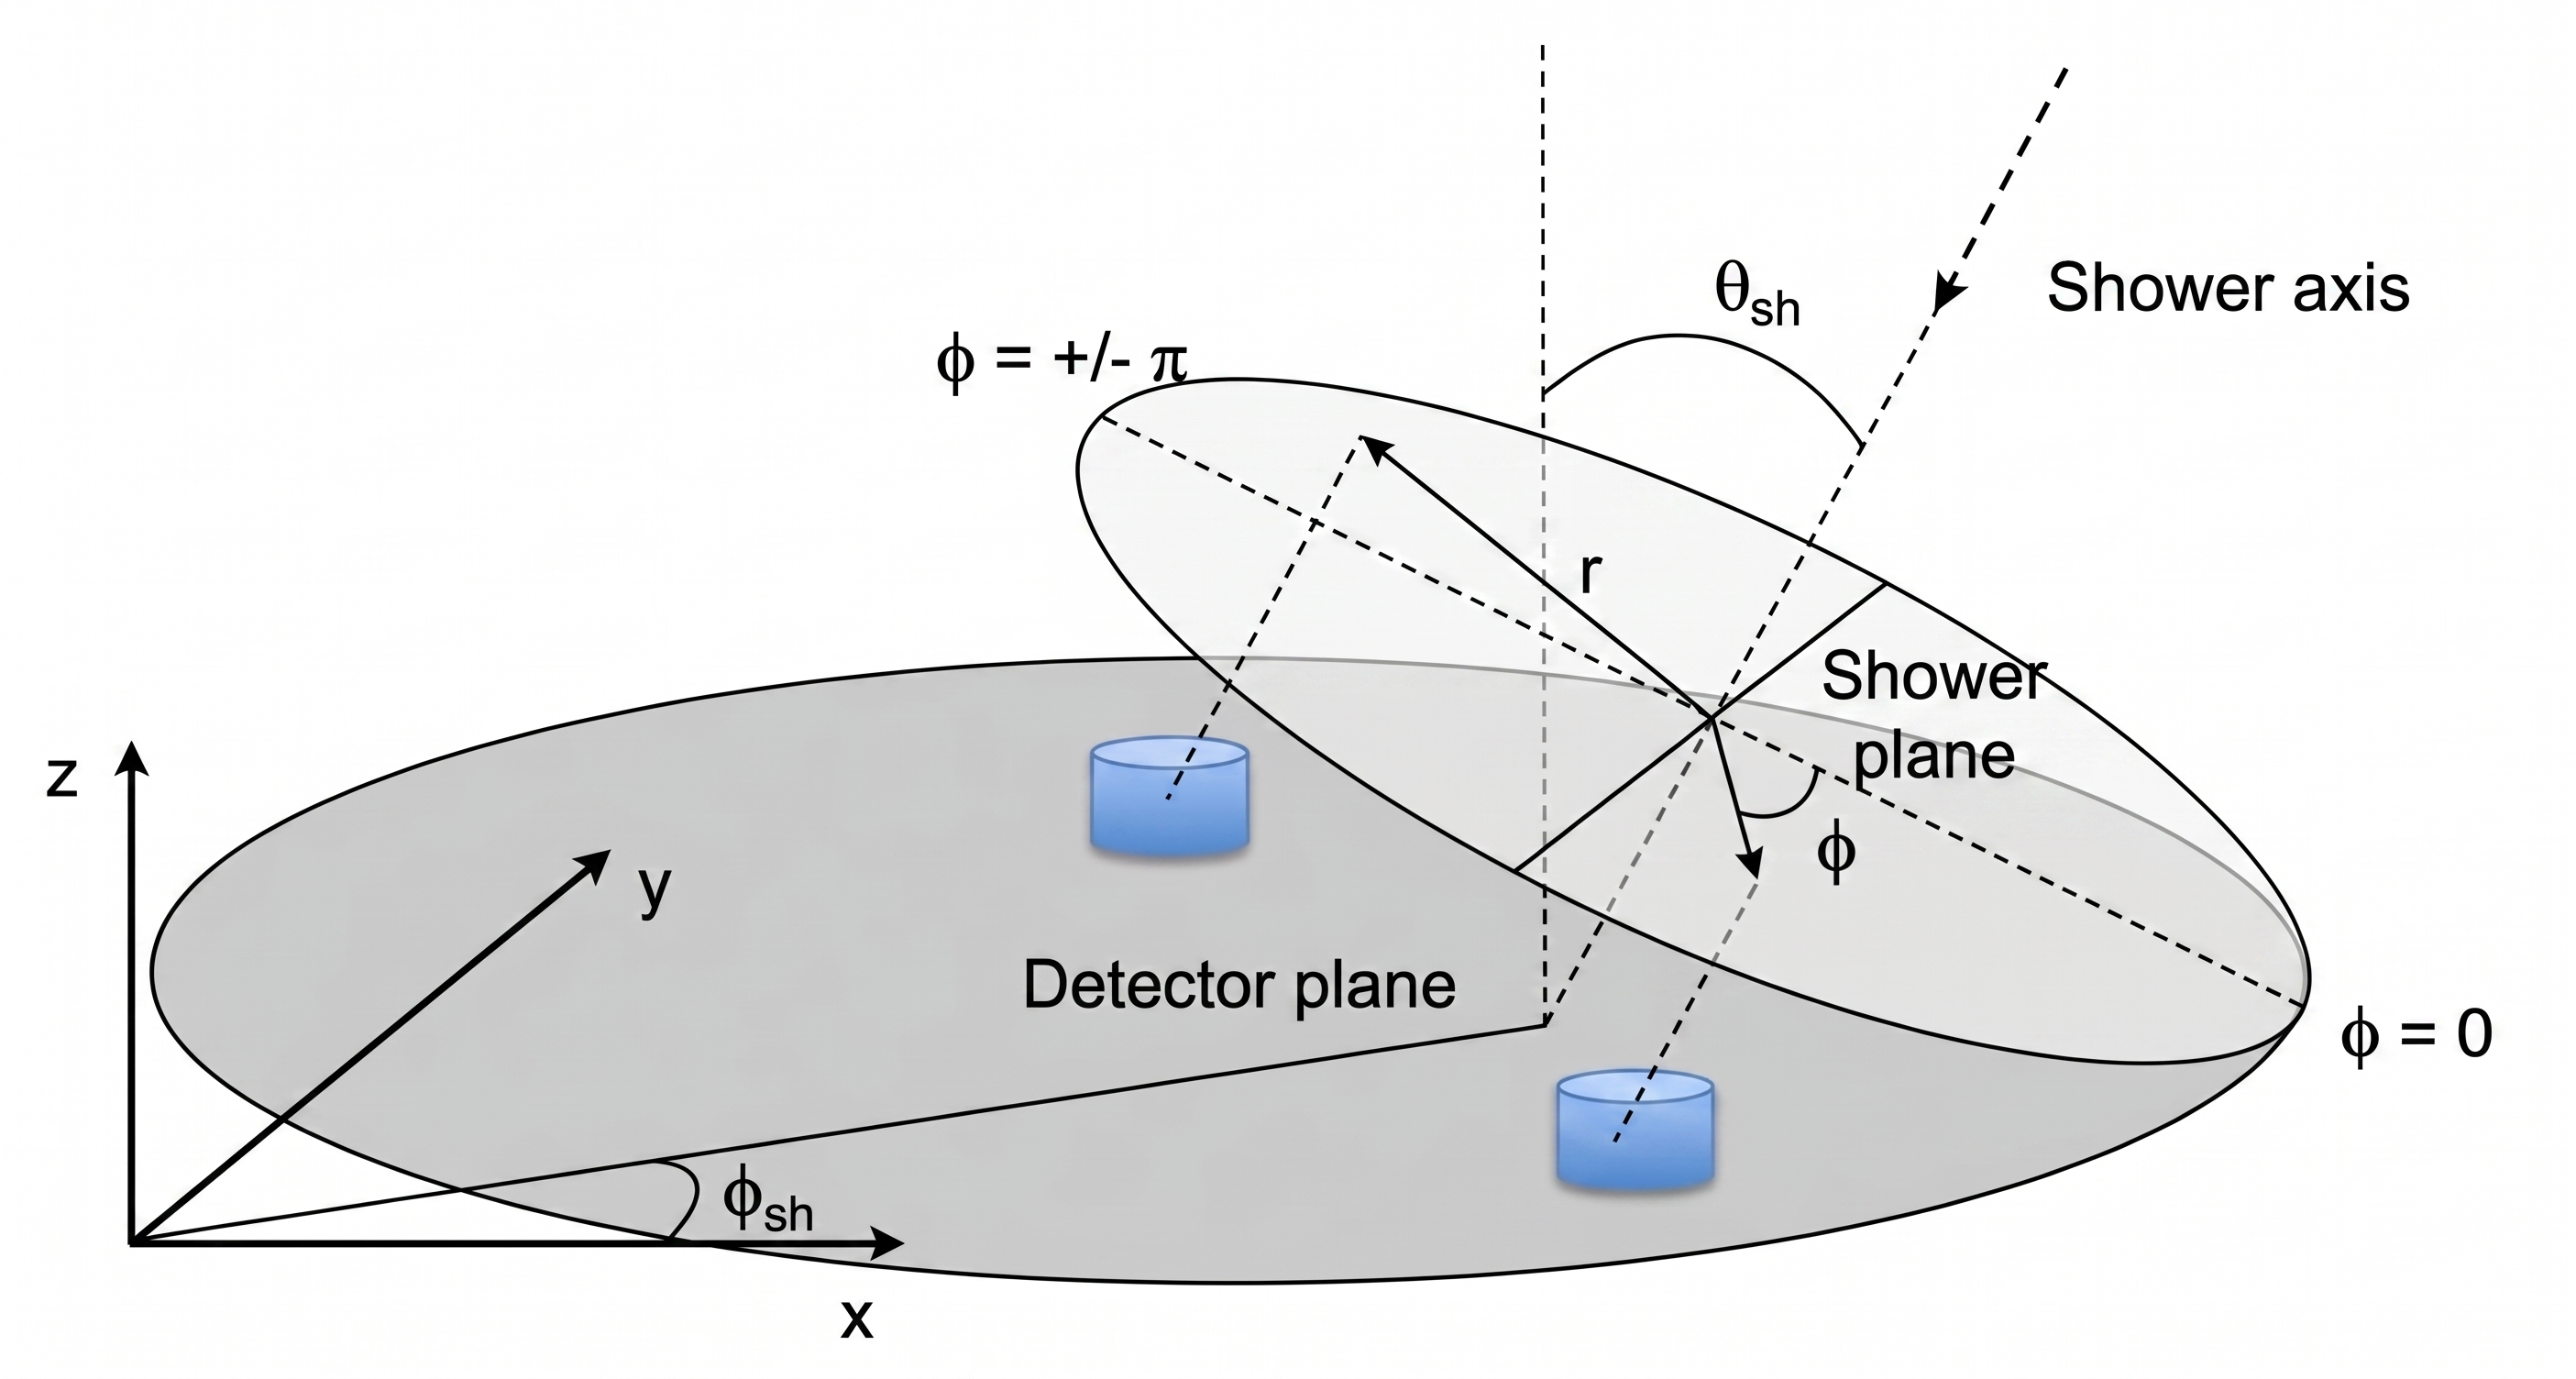
\includegraphics[width=\textwidth]{figuras/esquema_lluvia_gap.jpeg}
\caption{Esquema geométrico de una lluvia atmosférica extensa. Las posiciones de los detectores se proyectan desde el plano del suelo hacia el plano de la lluvia, donde se definen el radio $r$ y el ángulo azimutal $\phi$. Los ángulos $\theta_{\mathrm{sh}}$ y $\phi_{\mathrm{sh}}$ describen la orientación del eje; $\theta_{\mathrm{sh}}$ corresponde al cenital $\theta$ utilizado en el texto. Se reproduce el esquema empleado en la nota GAP asociada a este trabajo.}
\label{fig:plano_lluvia}
\end{figure}

En el caso ideal de una lluvia estrictamente vertical ($\theta=0^\circ$), ambos planos coinciden. Para un punto de producción sobre el eje, la distancia de vuelo hasta el suelo depende exclusivamente de la distancia radial al núcleo ($r$). Al extender esta construcción a una distribución de producción axialmente simétrica, los detectores ubicados a una misma distancia $r$ registrarán, en promedio y bajo las aproximaciones anteriores, idénticas densidades de muones, reflejando una simetría circular independiente del ángulo azimutal ($\phi$).

Sin embargo, cuando el rayo cósmico primario incide con un ángulo cenital $\theta>0^\circ$, el plano de la lluvia deja de ser paralelo al plano del suelo. Esta inclinación modifica las distancias de propagación respecto al observador terrestre.

Para comprender esta ruptura geométrica, es necesario analizar la intersección del frente de la lluvia con la superficie del arreglo. Al inclinar la cascada, estaciones situadas a igual radio $r$ en el plano de la lluvia pueden encontrarse a distintas distancias, medidas a lo largo de las trayectorias, de la región de producción de partículas. En particular, los dos extremos de la dirección temprano--tardía no se encuentran a la misma distancia de una fuente situada sobre el eje. Por ende, las partículas que componen la lluvia no recorren caminos idénticos antes de impactar contra el suelo. Esto define dos regiones azimutales fundamentales para el análisis de asimetrías:

\begin{itemize}
\item \textbf{Región temprana ($\phi\approx0^\circ$):} corresponde a la sección del frente de lluvia que se encuentra más cerca de la superficie topográfica y, por ende, impacta primero contra el arreglo de detectores. Para una misma fuente y un mismo radio $r$, las partículas que arriban a esta zona tienen el camino geométrico más corto y atraviesan menos atmósfera.
\item \textbf{Región tardía ($\phi\approx\pm180^\circ$):} corresponde a la sección diametralmente opuesta del frente, que se encuentra elevada respecto al suelo. Las partículas en esta dirección deben continuar propagándose después de que el lado temprano ha impactado, acumulando un trayecto atmosférico mayor antes de ser detectadas.
\end{itemize}

Esta diferencia de origen geométrico en las distancias de propagación, para un mismo radio $r$, interviene en los fenómenos físicos que modulan la densidad de muones. Los nombres temprano y tardío identifican posiciones respecto al eje de la lluvia, no retrasos individuales de los muones dentro de una misma estación.

\subsection{Origen físico de la modulación azimutal}
\label{subsec:origen_fisico}

La ruptura de la simetría circular resulta de mecanismos que actúan durante el desarrollo y la propagación de la cascada. Para comprender su competencia se describen primero la atenuación atmosférica, la proyección geométrica del flujo y la divergencia cinemática de la emisión. Luego se distingue esta física de propagación de la respuesta geométrica del detector.

\subsubsection{Atenuación atmosférica}
\label{subsubsec:atenuacion}

La atenuación es consecuencia de las pérdidas que experimentan las partículas durante su propagación. Como se estableció en la Sección~\ref{subsec:simetria_ruptura}, en una lluvia inclinada el trayecto hacia la región tardía es mayor que hacia la temprana. Para partículas con condiciones de producción equivalentes, ese recorrido adicional aumenta la posibilidad de decaer o de perder la energía necesaria para alcanzar el detector. Este mecanismo favorece, por lo tanto, un exceso temprano.

Una descripción analítica sencilla consiste en suponer que, en cada intervalo de recorrido $\mathrm dL$, se pierde una fracción constante de las partículas que aún sobreviven. Si $N(L)$ es su número, esta hipótesis se escribe
\[
\frac{\mathrm dN}{\mathrm dL}=-\frac{N}{\lambda},
\qquad
N(L)=N(0)e^{-L/\lambda}.
\]
La constante $\lambda>0$ tiene unidades de longitud: después de recorrer una distancia $\lambda$, permanece una fracción $e^{-1}$ de la población inicial. Ésta es la forma fenomenológica utilizada por Armbruster~\cite[Sec.~2.3.2, Ec.~(2.11)]{Armbruster2018},
\[
f_{\mathrm{att}}(L)=e^{-L/\lambda}.
\]
Su consecuencia para la asimetría se ve directamente al comparar ambos lados:
\[
\frac{f_{\mathrm{att}}(L_{\text{tardío}})}
     {f_{\mathrm{att}}(L_{\mathrm{temprano}})}
=\exp\!\left[-\frac{L_{\text{tardío}}-L_{\mathrm{temprano}}}{\lambda}\right]<1.
\]
Este cociente expresa una pérdida relativa del lado tardío. La exponencial caracteriza una contribución de atenuación; no incluye por sí sola la redistribución lateral de partículas ni su producción a distintas profundidades.

En los muones, una parte de esta pérdida tiene un origen concreto: el decaimiento en vuelo. La ley exponencial en el tiempo propio, junto con la dilatación temporal, da para un muón de velocidad y energía constantes
\[
P_{\mathrm{dec}}(L)=\exp\!\left[-\frac{L}{\beta_\mu\gamma_\mu c\tau_\mu}\right],
\qquad
\lambda_{\mathrm{dec}}=\beta_\mu\gamma_\mu c\tau_\mu.
\]
Aquí $\tau_\mu$ es la vida media propia, $\beta_\mu=v/c$ y $\gamma_\mu$ el factor de Lorentz. Se recupera así una exponencial en la distancia, pero con una longitud de decaimiento que depende de la energía del muón. La longitud efectiva $\lambda$ de Armbruster no se identifica automáticamente con un único valor de $\lambda_{\mathrm{dec}}$ para toda la población.

Si el muón pierde energía durante el vuelo, su longitud de decaimiento cambia a lo largo del recorrido. Dividiendo la trayectoria en pequeños intervalos y multiplicando sus probabilidades de supervivencia se obtiene
\[
P_{\mathrm{dec}}(L)=
\exp\!\left[-\int_0^L
\frac{\mathrm ds}{\beta_\mu(s)\gamma_\mu(s)c\tau_\mu}\right].
\]
La integral es, por tanto, la extensión de la misma ley de decaimiento cuando la energía deja de ser constante. En el límite relativista, $\beta_\mu\simeq1$ y $\gamma_\mu=E_\mu/(m_\mu c^2)$, se obtiene la tasa de decaimiento por unidad de longitud empleada en el transporte de Cazón \textit{et al.}~\cite[Sec.~3.2]{Cazon2012}. Las pérdidas de energía deben calcularse además para determinar si el muón llega al suelo y si conserva el alcance necesario para atravesar la cobertura del UMD.

La componente electromagnética posterior al máximo de la cascada suele ser más sensible al espesor atmosférico adicional que la componente muónica~\cite{Pryke1998,BradfieldThesis}. Sin embargo, el signo o la magnitud de la asimetría muónica observada no permiten afirmar, por sí solos, que la atenuación sea su contribución dominante. El suelo sobre el UMD filtra la energía y la dirección de los muones que llegan al centellador; este filtrado es posterior a la propagación atmosférica y debe distinguirse de ella~\cite{UMD_Design2016}.

\subsubsection{Efectos geométricos}
\label{subsubsec:divergencia}

El segundo grupo de mecanismos es de naturaleza geométrica y cinemática. Conviene separar dos aspectos: cómo un flujo local de partículas divergentes intercepta el plano del suelo, y cómo la distancia finita a la región de producción determina qué ángulos de emisión permiten alcanzar cada posición. El primero corresponde al término de proyección de Bertou y Billoir~\cite{GAP2000_017}; el segundo se desarrolla en la subsección siguiente.

\paragraph{Proyección geométrica del flujo.}

Las partículas no se desplazan todas paralelas al eje. Para un flujo que se abre radialmente hacia afuera, las trayectorias que alcanzan el lado temprano inciden más perpendicularmente sobre el suelo que las que alcanzan el lado tardío. Una superficie horizontal intercepta, por esa razón, un número diferente de partículas en ambas regiones. Proyectar después las posiciones al plano de la lluvia no elimina esa diferencia: la incidencia está determinada por la dirección de cada partícula, y no únicamente por la dirección del eje.

Bertou y Billoir expresan la modulación correspondiente como~\cite[Sec.~4, Ec.~(4)]{GAP2000_017}
\begin{equation}
\mathcal A_{\mathrm{geo}}(r,\phi)=
\left\langle\frac{p_r(r)}{-p_z(r)}\right\rangle_{\!\perp}
\tan\theta\cos\phi.
\label{eq:efecto_geo}
\end{equation}
El eje longitudinal se toma hacia arriba, por lo que $p_z<0$ para partículas descendentes respecto a ese eje. La componente $p_r$ es radial y tiene signo: es positiva para una trayectoria que se aleja del eje. El promedio indicado corresponde al flujo que cruza el plano perpendicular al eje. Para una población con divergencia radial media positiva, el coeficiente de $\cos\phi$ es positivo y esta contribución favorece la región temprana, al igual que las pérdidas descritas anteriormente.

En particular, reducir el momento longitudinal no invierte por sí mismo el signo de este término. Tampoco debe reemplazarse $p_r$ por el módulo del momento transversal si la población incluye direcciones radialmente entrantes. La expresión describe la proyección de un flujo divergente; no implica que un haz perfectamente paralelo al eje adquiera un dipolo simplemente por transformar sus coordenadas.

\subsubsection{Divergencia cinemática de la emisión de muones}
\label{subsubsec:divergencia_cinematica}

A diferencia del efecto de incidencia local, este mecanismo surge de comparar, para una misma distancia radial $r$ en el plano de la lluvia, la distancia física $d$ que un muón debe recorrer desde su punto de producción hasta alcanzar la región temprana o la tardía.

Para comprenderlo es necesario analizar primero la cinemática de producción de muones. En la cascada hadrónica, los muones se producen principalmente en decaimientos de piones y kaones. Se considera inicialmente una fuente situada a una distancia $D$ del núcleo, medida sobre el eje de la lluvia. Los muones heredan un momento longitudinal y un momento transversal $p_t$, que determina su ángulo de emisión $\alpha$ respecto al eje. Si $p$ es el módulo del momento y $E$ la energía total de producción, se cumple
\[
p_t=p\sin\alpha,
\qquad
\sin\alpha\simeq\frac{cp_t}{E}
\quad\text{para }E\gg m_\mu c^2.
\]
La fuente puntual permite visualizar la geometría; en una lluvia real, los muones se producen a distintas profundidades y con una distribución de energías y momentos transversales~\cite{Cazon2012}.

Al propagarse las partículas hacia el suelo, su densidad depende de dos factores que compiten entre sí. Por un lado, un mismo elemento de ángulo sólido cubre un área mayor al aumentar la distancia: para una superficie perpendicular a la trayectoria, $\mathrm dA_\perp=d^2\mathrm d\Omega$. Por ello, la densidad disminuye como $1/d^2$. Por otro lado, el número de partículas emitidas por unidad de ángulo sólido depende del ángulo $\alpha$ exigido para alcanzar esa posición. Antes de incorporar pérdidas e incidencia sobre el detector, esta densidad se escribe
\begin{equation}
S_\perp(d,\alpha)\propto\frac{1}{d^2}\frac{\mathrm dN}{\mathrm d\Omega}(\alpha).
\label{eq:asym_a1_previa}
\end{equation}
El subíndice recuerda que se trata de una densidad por área normal a la trayectoria. Para convertirla en conteo en una placa o en señal del SD debe incluirse la respuesta correspondiente, que se discute más adelante.

Como aproximación al espectro transversal, se adopta la forma
\[
\frac{\mathrm dN}{\mathrm dp_t}\propto p_t\exp(-p_t/Q),
\]
donde $Q$ es una escala de momento. Cazón \textit{et al.} discuten esta parametrización y las limitaciones de tratarla como independiente de la energía y de la profundidad de producción~\cite[Sec.~2]{Cazon2012}. Aquí se la utiliza para mostrar cómo el espectro transversal se traduce en una distribución de ángulos.

A energía fija y suponiendo simetría azimutal alrededor del eje, $\mathrm d\Omega=2\pi\sin\alpha\,\mathrm d\alpha$ y $\mathrm dp_t=p\cos\alpha\,\mathrm d\alpha$. El cambio de variables da
\[
\frac{\mathrm dN}{\mathrm d\Omega}
=\frac{\mathrm dN}{\mathrm dp_t}\frac{\mathrm dp_t}{\mathrm d\Omega}
\propto p_t e^{-p_t/Q}\frac{p\cos\alpha}{2\pi\sin\alpha}
\propto p^2\cos\alpha\,e^{-p\sin\alpha/Q}.
\]
El factor $p_t$ del espectro se cancela con el que proviene del ángulo sólido. En el límite relativista, la dependencia angular resultante es
\begin{equation}
\frac{\mathrm dN}{\mathrm d\Omega}(\alpha\mid E)
\propto\cos\alpha\,\exp\!\left(-\frac{E\sin\alpha}{cQ}\right).
\label{eq:cazon_dNdOmega}
\end{equation}
En esta proporcionalidad se ha omitido un factor constante respecto a $\alpha$, pero dependiente de $E$. Se lo recuperará al combinar muones de distintas energías.

En una lluvia inclinada, alcanzar un mismo radio $r$ requiere un recorrido mayor hacia la región tardía que hacia la temprana ($d_{\text{tardío}}>d_{\mathrm{temprano}}$). Por lo tanto, el ángulo de emisión requerido es menor del lado tardío ($\alpha_{\text{tardío}}<\alpha_{\mathrm{temprano}}$): para llegar al mismo desplazamiento transversal recorriendo menos distancia, el muón temprano debe apartarse más del eje. Esta construcción se ilustra en la Figura~\ref{fig:divergencia_angular}.

\begin{figure}[H]
\centering
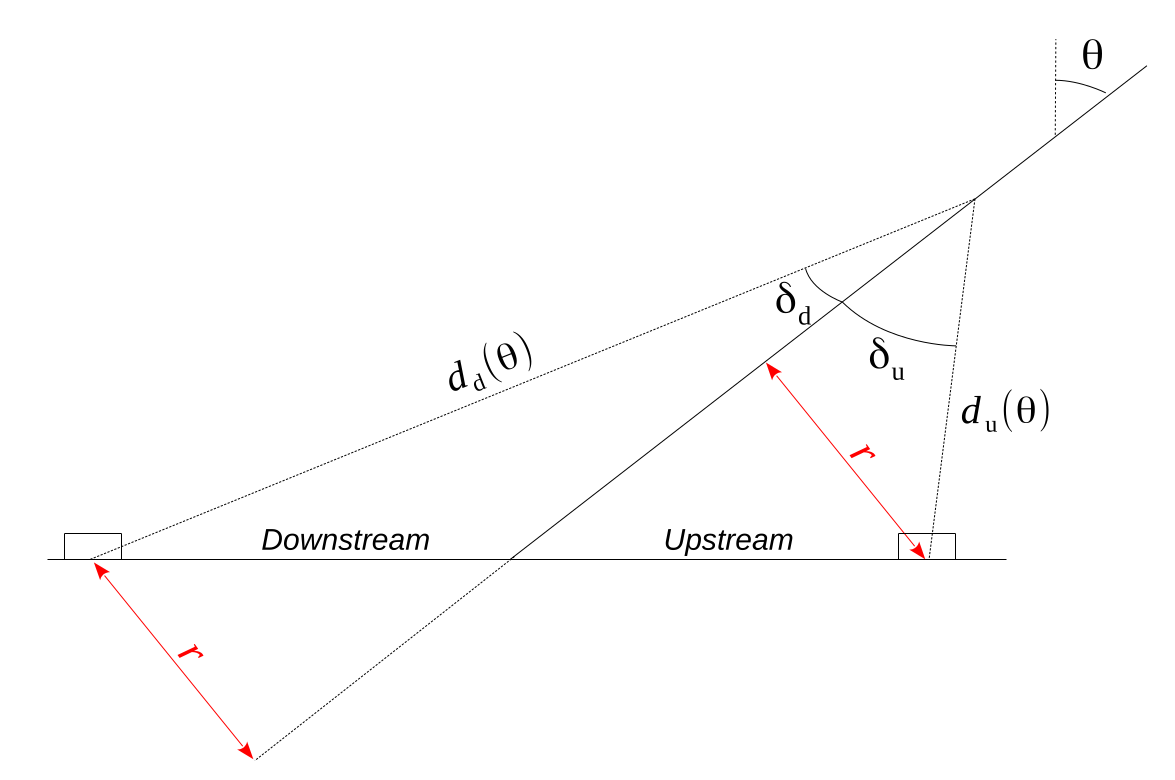
\includegraphics[width=\textwidth]{figuras/efecto_geo_luce_icrc2021.png}
\caption{Geometría de emisión hacia las regiones temprana y tardía a igual radio en el plano de la lluvia. El ángulo requerido hacia el lado tardío ($\delta_d$ en la figura) es menor que hacia el temprano ($\delta_u$). Tomado de~\cite{Luce_ICRC2021}.}
\label{fig:divergencia_angular}
\end{figure}

Para calcular ambos recorridos sin mezclar el radio del suelo con el radio de la lluvia, la geometría de una fuente sobre el eje da
\[
d(\phi)=\sqrt{\bigl(D-r\tan\theta\cos\phi\bigr)^2+r^2},
\qquad
\sin\alpha(\phi)=\frac{r}{d(\phi)}.
\]
Se consideran posiciones aguas abajo de la fuente, $D>r\tan\theta$. En particular, el desplazamiento axial es proporcional a $r\tan\theta$, porque $r$ está definido en el plano de la lluvia~\cite[Sec.~2.2.2]{Armbruster2018}.

Combinando las Ecs.~\ref{eq:asym_a1_previa} y~\ref{eq:cazon_dNdOmega}, el cociente entre las dos regiones, a una misma energía de producción, resulta
\begin{equation}
\begin{split}
\frac{S_{\perp,\text{tardío}}}{S_{\perp,\mathrm{temprano}}}
\simeq{}&
\underbrace{\left(\frac{d_{\mathrm{temprano}}}{d_{\text{tardío}}}\right)^2}_{\text{dilución espacial }<1}
\quad\underbrace{\frac{\cos\alpha_{\text{tardío}}}{\cos\alpha_{\mathrm{temprano}}}}_{\text{factor angular }>1}
\\[-1pt]
&\times\underbrace{\exp\!\left[
\frac{(\sin\alpha_{\mathrm{temprano}}-\sin\alpha_{\text{tardío}})E}{cQ}
\right]}_{\text{preferencia por el ángulo menor }>1}.
\end{split}
\label{eq:asym_kinematic_ratio}
\end{equation}

El primer factor favorece al lado temprano: la mayor distancia tardía distribuye las partículas sobre un área mayor. Los dos factores angulares favorecen al lado tardío: para llegar allí se necesita una dirección más próxima al eje, donde la distribución de emisión es más poblada. El cociente expresa esa competencia. Puede ser mayor o menor que uno según los parámetros; no basta con que la contribución angular favorezca el lado tardío para concluir que supera a la dilución. Hasta aquí se compararon muones de una misma energía, emitidos desde una misma distancia, sin atenuación ni respuesta instrumental.


\subsubsection{Cómo combinar muones de distintas energías}
\label{subsubsec:promedio_energetico}

Una lluvia contiene muones de muchas energías. Para extender la Ec.~\ref{eq:asym_kinematic_ratio} a esa población, el primer paso es sumar cuántos llegan al lado temprano y cuántos al tardío. El cociente se calcula después de efectuar ambas sumas. Promediar directamente los cocientes de cada energía con el espectro de producción no realiza esa operación.

Sea $G(E)\,\mathrm dE$ el número de muones producidos en un intervalo de energía, manteniendo por ahora una misma distancia de producción $D$. Denotamos por $f(\alpha\mid E)$ la distribución angular \emph{normalizada}: $f(\alpha\mid E)\,\mathrm d\Omega$ es la probabilidad de que un muón de esa energía sea emitido dentro del elemento de ángulo sólido considerado. Su contribución a la densidad de una región $j$ es
\[
\mathrm dS_{\perp,j}(E)=G(E)\,\mathrm dE\,
\frac{f(\alpha_j\mid E)}{d_j^2},
\qquad j=\text{temprano, tardío}.
\]
Se distinguen así dos ingredientes: cuántos muones se producen a una energía determinada y qué fracción se emite en la dirección necesaria para alcanzar esa región. La distribución angular puede ser la misma función en ambos lados, pero se evalúa en dos ángulos distintos. Por ello, el espectro de producción no es, en general, el espectro de los muones que llegan a cada posición.

El cociente correcto de densidades integradas es
\begin{equation}
\frac{\overline S_{\perp,\text{tardío}}}
     {\overline S_{\perp,\mathrm{temprano}}}
=\left(\frac{d_{\mathrm{temprano}}}{d_{\text{tardío}}}\right)^2
\frac{\displaystyle\int G(E)f(\alpha_{\text{tardío}}\mid E)\,\mathrm dE}
     {\displaystyle\int G(E)f(\alpha_{\mathrm{temprano}}\mid E)\,\mathrm dE}.
\label{eq:cociente_espectro}
\end{equation}
La barra indica aquí la suma sobre energías. Los límites de integración deben corresponder a la población de producción que se esté modelando.

Hay una segunda precaución. La Ec.~\ref{eq:cazon_dNdOmega} sólo indicaba la forma angular a energía fija. Para usarla en la Ec.~\ref{eq:cociente_espectro} es necesario escribir
\[
f(\alpha\mid E)=C(E)\cos\alpha\,
\exp\!\left(-\frac{E\sin\alpha}{cQ}\right),
\qquad \int f(\alpha\mid E)\,\mathrm d\Omega=1.
\]
La constante $C(E)$ depende de la energía porque una distribución más colimada concentra la misma probabilidad en un ángulo sólido menor. Se cancela al comparar temprano y tardío a una sola energía, pero debe conservarse al sumar energías distintas.\footnote{En la aproximación relativista de la Ec.~\ref{eq:cazon_dNdOmega}, normalizada en el hemisferio delantero, $C(E)=k^2/\{2\pi[1-(1+k)e^{-k}]\}$, con $k=E/(cQ)$. Fuera de ese límite debe usarse $k=p/Q$, con $pc=\sqrt{E^2-m_\mu^2c^4}$. Esta normalización corresponde al espectro transversal supuesto y restringido a $0\leq p_t\leq p$; no constituye por sí misma un modelo completo de producción.}

La supervivencia durante el vuelo puede incorporarse multiplicando cada contribución por su probabilidad de supervivencia antes de integrar. Del mismo modo, la predicción de un conteo o de una señal requiere incluir su respuesta instrumental. Una fuente extendida exige además sumar sobre las profundidades de producción, conservando sus correlaciones con la energía. En particular, el umbral del UMD actúa sobre el muón que alcanza el suelo: no debe introducirse como un corte idéntico sobre su energía de producción sin modelar antes el transporte. Estas extensiones permiten plantear un cálculo cuantitativo, pero la Ec.~\ref{eq:asym_kinematic_ratio} aislada no determina cuál de los dos detectores tendrá una asimetría mayor.

\subsubsection{Qué cambia al medir señal en un tanque de agua}
\label{subsubsec:respuesta_tanque}

La geometría del detector interviene después de que las partículas han llegado a su entorno. Para un mismo flujo incidente, un tanque puede recibir partículas por la tapa y por los laterales. Como las direcciones de incidencia temprana y tardía son diferentes, también puede cambiar el área que el tanque presenta a esas partículas.

Sin embargo, en la señal muónica hay otro factor: cada muón que atraviesa el agua produce una señal aproximadamente proporcional a la longitud de su trayectoria dentro del tanque. Cambiar la dirección de incidencia modifica tanto cuántos muones interceptan el volumen como la longitud media que recorren en él. Ambos factores se compensan en el límite ideal de muones pasantes, como discuten Bertou y Billoir~\cite[Sec.~6]{GAP2000_017}, Billoir, Da Silva y Bertou~\cite[Sec.~2]{GAP2002_074} y Armbruster~\cite[Sec.~2.4]{Armbruster2018}.

Para visualizar esta compensación, se puede imaginar el volumen de agua dividido en haces delgados, todos paralelos a una dirección incidente. Cada haz ocupa un área transversal $\mathrm dA_\perp$ y atraviesa una longitud $\ell$ de agua. Su volumen es $\ell\,\mathrm dA_\perp$. Al sumar todos los haces se recupera el volumen total $V$, cualquiera sea la dirección elegida. Por lo tanto,
\begin{equation}
A_{\mathrm{ef}}\,\langle\ell\rangle=V,
\label{eq:compensacion_tanque}
\end{equation}
donde $A_{\mathrm{ef}}$ es el área proyectada del tanque sobre un plano normal a esa dirección y $\langle\ell\rangle$ la longitud media de las trayectorias que lo atraviesan. Una mayor área efectiva se acompaña de una menor longitud media; no son dos ganancias independientes que puedan multiplicarse sin esta relación.

Si $F_\perp$ es el número de muones incidentes por unidad de área normal a su dirección y $q$ la señal producida por unidad de recorrido, entonces
\begin{equation}
N_\mu=F_\perp A_{\mathrm{ef}},
\qquad
S_\mu=q\,N_\mu\langle\ell\rangle
=q\,F_\perp V.
\label{eq:senal_muonica_tanque}
\end{equation}
La respuesta por unidad de flujo depende del volumen de agua, pero ya no del ángulo a través de $A_{\mathrm{ef}}$. Esto no hace iguales las señales temprana y tardía si el propio flujo $F_\perp$ es diferente en ambas regiones. La compensación elimina la contribución angular de la respuesta ideal del tanque, no la asimetría producida durante la propagación de la lluvia.

La distinción con el conteo también es importante: contar muones da $N_\mu$, sin el factor de longitud de traza que aparece en la señal. Para ese observable, el área efectiva sigue interviniendo. La compensación anterior supone un flujo aproximadamente uniforme sobre la escala del tanque, muones que lo atraviesan y una señal lineal en la longitud recorrida. Los muones que se detienen, los efectos de respuesta óptica y los requisitos de selección requieren un tratamiento adicional. Tampoco corresponde aplicar esta cancelación muónica a toda la señal electromagnética del SD.

\subsubsection{Conexión con el modelo de Armbruster}
\label{subsubsec:conexion_armbruster}

Los elementos anteriores permiten recuperar de manera directa la expresión utilizada por Armbruster y retomada por Luce \textit{et al.}~\cite{Armbruster2018,Luce_ICRC2021}. Para una fuente efectiva sobre el eje, con atenuación exponencial y la respuesta ideal de señal muónica recién descrita, los factores variables con el azimut son
\begin{equation}
S_\mu(\phi)\propto
\underbrace{\frac{1}{d(\phi)^2}}_{\text{dilución}}
\quad\underbrace{f\bigl(\alpha(\phi)\bigr)}_{\text{distribución angular}}
\quad\underbrace{e^{-d(\phi)/\lambda}}_{\text{atenuación}}.
\label{eq:producto_armbruster}
\end{equation}
El volumen del tanque y la conversión de longitud de traza a señal son constantes y quedan incluidos en la normalización. Armbruster aproxima la distribución angular por una potencia, $f(\alpha)\propto\alpha^{-\gamma_{\mathrm{ADF}}}$. El parámetro $\gamma_{\mathrm{ADF}}$ es la pendiente de esa distribución; no es el factor de Lorentz del muón ni una longitud de atenuación.

Para ver cómo aparece la asimetría, se toma $r/D\ll1$ y se define $\varepsilon=(r/D)\tan\theta$. A primer orden en la pequeña diferencia de recorridos entre ambos lados,
\[
d(\phi)\simeq D(1-\varepsilon\cos\phi),
\qquad
\alpha(\phi)\simeq\frac{r}{D}(1+\varepsilon\cos\phi).
\]
Cada factor de la Ec.~\ref{eq:producto_armbruster} aporta entonces una modulación sencilla:
\begin{align*}
\frac{1}{d(\phi)^2}&\simeq\frac{1}{D^2}
\bigl[1+2\varepsilon\cos\phi\bigr],
\\
f\bigl(\alpha(\phi)\bigr)&\simeq f(r/D)
\bigl[1-\gamma_{\mathrm{ADF}}\varepsilon\cos\phi\bigr],
\\
e^{-d(\phi)/\lambda}&\simeq e^{-D/\lambda}
\bigl[1+(D/\lambda)\varepsilon\cos\phi\bigr].
\end{align*}
Estas expansiones requieren $|\varepsilon|\ll1$ y una variación pequeña de los factores; en particular, $r\tan\theta/\lambda\ll1$ y $|\gamma_{\mathrm{ADF}}\varepsilon|\ll1$. Al multiplicarlas y conservar sólo el primer orden, se obtiene
\begin{equation}
\frac{S_\mu(\phi)}{S_{\mu,0}}\simeq
1+\left(2-\gamma_{\mathrm{ADF}}+\frac{D}{\lambda}\right)
\frac{r}{D}\tan\theta\cos\phi.
\label{eq:amplitud_armbruster}
\end{equation}
El coeficiente de $\cos\phi$ coincide con la Ec.~(2.33) de Armbruster, identificando su distancia axial $d$ con nuestro $D$. El término $+2$ procede de la dilución, el término $-\gamma_{\mathrm{ADF}}$ de la preferencia por ángulos menores y el término $D/\lambda$ de la atenuación. Así se recupera, con otra elección para la distribución angular, la misma competencia física descrita anteriormente.

No se añade aquí un término separado de proyección de placa: se está calculando la señal ideal del tanque, cuya apertura angular ya se compensó con la longitud media de traza. La comparación muestra la consistencia del esquema con la bibliografía; no determina los parámetros efectivos de una población real ni constituye un ajuste a los resultados de esta tesis.

\subsubsection{Efectos por el campo geomagnético terrestre}
\label{subsubsec:geomagnetico}

Finalmente, la simetría se ve alterada por la acción de la fuerza de Lorentz sobre la componente cargada de la lluvia. El campo geomagnético terrestre ($\vec B$) desvía las trayectorias según $\vec F=q\vec v\times\vec B$, separando lateralmente a muones de cargas opuestas ($\mu^+$ y $\mu^-$). La desviación aumenta al disminuir la rigidez y al aumentar el recorrido, por lo que adquiere especial relevancia en lluvias muy inclinadas~\cite{collaboration_2014,Cazon2012}.

La orientación de esta distorsión depende de la dirección de llegada de la lluvia respecto al campo y no coincide, en general, con el eje temprano--tardío. Promediar distintas direcciones de arribo puede reducir algunas contribuciones, pero no garantiza su cancelación ni una disminución sistemática de la amplitud temprano--tardía. La propagación rectilínea usada en las derivaciones anteriores omite este efecto, así como la dispersión múltiple. Esas aproximaciones delimitan el alcance del modelo analítico y deben distinguirse del transporte incluido en las simulaciones.

\subsection{La selección de estaciones y el promedio medido}
\label{subsec:respuesta_seleccion}

Los mecanismos anteriores describen la llegada de partículas y la respuesta del detector. Para relacionarlos con un perfil medido queda una cuestión distinta: sobre qué estaciones se calcula el promedio. El conteo medio de todas las estaciones simuladas de un intervalo no tiene por qué coincidir con el de las estaciones que satisfacen un requisito de disparo o de reconstrucción.

Si ese requisito favorece a estaciones con más muones, la media de las retenidas aumenta aunque ningún conteo individual haya cambiado. Si la preferencia es diferente entre temprano y tardío, también puede cambiar la asimetría de la media seleccionada. Una pérdida aleatoria reduce la estadística disponible sin cambiar sistemáticamente la media; un cambio sistemático requiere que la selección esté relacionada con el conteo o con variables correlacionadas con él.

Esta distinción sigue siendo necesaria al utilizar conteos de verdad Monte Carlo: conocer exactamente los muones de una estación no asegura que el conjunto de estaciones retenidas sea representativo. Comparar los conteos antes y después de la condición de selección SD permite evaluar este efecto en el \textit{Infill}; su desarrollo corresponde al capítulo dedicado a ese arreglo. Aquí se introduce únicamente para distinguir una modulación de la población incidente de una modulación del promedio calculado sobre una muestra seleccionada.

\subsection{Parametrización armónica de primer orden}
\label{subsec:parametrizacion}

Para cuantificar la modulación azimutal, se utiliza la parametrización armónica de primer orden empleada en estudios del Detector de Superficie~\cite{Billoir2002,BradfieldThesis}:
\begin{equation}
S(r,\phi)=S_0(r)\bigl[1+A_1(r,\theta)\cos\phi\bigr].
\label{eq:asimetria_a1}
\end{equation}
La magnitud $S$ representa la densidad, el conteo medio o la señal, según el observable que se declare en cada análisis. $S_0$ es su normalización azimutal, y $A_1$ es un coeficiente con signo. Un valor $A_1>0$ indica un exceso temprano; un valor $A_1<0$, un exceso tardío. El signo caracteriza el resultado de la competencia de contribuciones, sin identificar por sí solo cuál de ellas domina.

Fijar el eje de la modulación en $\phi=0$ permite estudiar la componente temprano--tardía, pero no obliga a que $A_1$ sea positivo. La posible presencia de una componente en $\sin\phi$ o de armónicos superiores debe evaluarse con los perfiles y los residuos del ajuste. Asimismo, sólo para una modulación puramente cosinusoidal se cumple exactamente $A_1=[S(0)-S(\pi)]/[S(0)+S(\pi)]$; comparar dos direcciones de un modelo no sustituye, en general, un ajuste al perfil completo.

Los capítulos siguientes utilizan este coeficiente para caracterizar las asimetrías del UMD y del SD y su dependencia con los parámetros de la lluvia. Su interpretación requiere mantener identificados el observable de cada detector, el transporte de las partículas que lo producen y la selección de estaciones sobre la que se calcula su promedio.

